\documentclass[a4paper,12pt]{article}
\title{CS 4102 Written HW4 - Dynamic Programming}
\author{Eric Xie}
\usepackage{graphicx}
\graphicspath{ {images/} }
\usepackage{listings}
\begin{document}
\maketitle
\noindent \textbf{1.} \\
Let f(n,s, L) be the solution to the problem with doors 1 through n and s doors need to be secured. Let L = 1 denote door n is locked and L = 0 denote door n is unlocked.\\
The last door can either be locked or unlocked. \\
Locked: f(n, s, 1)\\
1) Door n-1 is unlocked, solve the subproblem f(n-1, s, 0)\\
2) Door n-1 is locked, solve the subproblem f(n-1, s-1, 1)\\
Unlocked: f(n, s, 0)\\
1) Door n-1 is unlocked, solve the subproblem f(n-1, s, 0)\\
2) Door n-1 is locked, solve the subproblem f(n-1, s, 1)\\
Therefore, there are 4 distinct configurations of the last 2 doors, and their subproblems must be added to find the total distinct ways to get S secured doors\\\\
Instantiate an n x S array. \\\\
\begin{lstlisting}
def f(n,s):
   If n<S: return 0 
   If n==s: return  1
   If s==0: return fib(n), where fib(0)=fib(1)=1
   If n==2, s==1: return 1
   if(arr[n][s])
      return arr[n][s];
   else
      return f(n-1, s, 0)+f(n-1, s-1, 1)+f(n-1, s, 0)+f(n-1, s, 1)
\end{lstlisting}

\noindent \textbf{2.} \\
For the brute-force method, simply try every possible starting point i and j for strings A and B with every substring length L. $SQ(i,j,L) < I$ and L is longer than the current solution, store it. \\
\begin{lstlisting}
Given words A, B, and int I, return L
n = len(A)
max = 0;
for i in [0,n):
   for j in [0,n):
      maxLen = n-max(i,j)
      for k in [1,maxLen]:
         if SQ(i,j,k)<=I && k>max:
	    max=k
def SQ(i,j,k):
   s1=A.substring(i,i+k)
   s2=B.substring(j,j+k)
   errors=0;
   for i in [0,k):
      if(s1[i]!=s2[i])
	errors++
  return errors
\end{lstlisting}
Runtime: $O(n^4)$, assuming SQ is O(n) \\\\
\noindent \textbf{3.} \\
This improved solution still iterates through every starting point i and j, but not every length L. Instead, we compare the two words at the current index and increment the substring length until we run out 
of bounds or we encounter I errors. For each i and j, the max length L is saved in arr[i][j].  
\begin{lstlisting}
Given words A, B, and int I, return L
n = len(A)
Instantiate an n x n array
max = 0;
for i in [0,n):
   for j in [0,n):
      maxLen = n-max(i,j)
      errors=0;
      for k in [0,maxLen]:
         if(A[i+k]!=B[j+k])
	    errors++
	 if(errors==L)
	    if(k>max)
		max=k;
	    break
\end{lstlisting}
The solution can be further improved. If the longest substring we can possible make starting from i and j is shorter than the longest substring within I errors, we can stop iterating. \\
Runtime = $O(n^3)$\\\\
\noindent \textbf{4.} \\
Given set of boxes B, return max number of boxes that can be placed inside one another\\
First, sort B by ascending volume, where volume=width, height, depth\\
Let arr[i]=The max number of boxes that fit inside box i, including box i itself. \\
The base solution, which is 1 box, is obvioulsy 1. arr[0]=1\\
As we add the ith box, which is always greater in volume than earlier boxes, it can possibly fit one of the earlier boxes.\\
In order to maximize boxes, we want the ith box to hold box j such that $j<i$ arr[j] is maximum. Thus we iterate from the 0th to jth box. \\
If the jth box fits inside box i, and arr[j] is maximal, then arr[i]=arr[j]+1\\
Next, instantiate an array of size n, where n is the number of boxes\\
\begin{lstlisting}
for i in [0,n):
   if(n==0)
	return 1
   else:
	temp = 0;
    	for j in (0,i):
	   if(fitsInside(B[j],B[i])):
	      temp=max(temp,arr[j])
      	arr[i]=temp+1
\end{lstlisting}
To find the actual set of boxes, we first identify the box that contains the most boxes, store its index in maxIndex, and append it to the solution set. Iterating backward from maxIndex, if a box contains 1 less than the maxIndex box, it is part of the solution set, and we set that box as maxIndex. 
\begin{lstlisting}
maxIndex=0
for i in [0,n):
   if(arr[i]>arr[maxIndex]):
	maxIndex=i;
solnBoxes=[]
solnBoxes.append(B[maxIndex])
for i in (maxIndex,0):
   if(arr[i]=arr[maxIndex]-1)
      maxIndex=i;
      solnBoxes.append(B[i])
\end{lstlisting}
Runtime = $O(n^2)$ to calculate each arr[i], $O(n)$ to find the solution set of boxes\\
However, if searching for the jth box for which arr[j] is maximal can be done in O(logn), then the overall runtime can be O(nlogn)\\\\
\noindent \textbf{5.} \\
Since the first priority is to complete all runs in the minimum number of days, use a greedy algorithm to find the number of days. \\
\begin{lstlisting}
days=0
minutes=0;
for i in (0,R.length):
   minutes+=R[i];
   if(minutes>=L)
      minutes-=L
      days++
\end{lstlisting}
Now we will try to minimize the total twd, which we store in a days x n array. Let arr[d][r] be the total twd accumulated when the last run on day d is run r.\\
We also know that the last run, R[n] must happen on the last day.\\
This means that the last run on the second to last day could be any run j such that $j<n$\\
arr[d][n] is thus the minimum twd of from the previous day plus the twd for just day d if the last run is run n. \\
The base case is day 1, which we have to calculate twd for every run up till the n-days run, because there must be at least 1 run on the remaining days. \\
Let n = R.length \\
Initialize an n x Days array. \\
\begin{lstlisting}
minutes=0;
for i in (0,n-days+1):
   minutes+=R[i];
   if(minutes<=L)
      arr[0][i]=twd(L-minutes)
   else:
      break
def f(day, run):
   min = Integer.MAX
   for j in (0, run-1):
      if(arr[day-1][j]):
         temp=arr[day-1][j]
      else:
         fn(day-1,j)
	 temp=arr[day-1][j]
      if(temp<min):
	 min=temp
f(Days,n)
\end{lstlisting}
The last run of each day can then be found by looping through the days. The minimum value in each column is the last run for that day. \\\\
\noindent \textbf{6.} \\
Initialize an array of size n \\
Base case: 
There is 1 way to tile a 2x1 grid
There are 2 ways to tile a 2x2 grid
\begin{lstlisting}
arr[1]=1
arr[2]=2
def tile(n):
   if(arr[n]):
	return arr[n]:
   else:
	return arr[n-1]+arr[n-2]
\end{lstlisting}
Runtime = $O(n)$, same as fibonacci \\\\
\noindent \textbf{7.} \\
There are 5 ways to tile the beginning of the board without leaving any incomplent rows. They are shown below as patterns A-E:\\
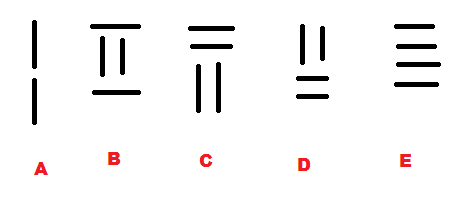
\includegraphics{simple}\\
Since A essentially solves 1 row, the total number of ways to tile the remainder of the board is the subproblem for n-1\\
Since B-E essentially solves 2 rows, the total number of ways to tile the remainder of the board is the subproblem for n-2\\
There are 3 more ways to tile the beginning of the board, but they result in an incomplete row. They are shown below as patterns F-H\\
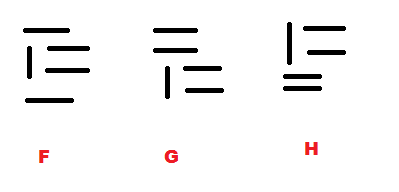
\includegraphics{complex}\\
If F is used, only a variation of B or F can be used to complete it. F solves 2 rows, but the remaining n-2 subproblem must start with B or F. \\
If G is used, it can only be completed by a variation of A, D, or H. G solves 2 rows, but the remaining n-2 subproblem must start with A, D, or H.\\
If H is used, it can only be completed by a variation of A, C, or G. H solves 2 rows, but the remaining n-2 subproblem must start with A, C, or G. \\\\
Let $f_L(n)$ be the number of ways to tile a 4 x n board starting with pattern L such that $L\in\{A-H\}$\\
Let $f(n)$ the total number of ways to tile a 4 x n board\\
Thus $f(n)=f_A(n)+f_B(n)+f_C(n)+f_D(n)+f_E(n)+f_F(n)+f_G(n)+f_H(n)$\\
Substituting in with the subproblems, we get:\\
$f(n)=f(n-1)+4f(n-2)+f_B(n-2)+f_F(n-2)+f_A(n-2)+f_D(n-2)+f_H(n-2)+f_A(n-2)+f_C(n-2)+f_G(n-2)$\\
We are adding the n-2 subproblem for every pattern except E, so it's easier to add $f(n-2)$ and subtract $f_E(n-2)$. Thus we have:\\
$f(n)=f(n-1)+5f(n-2)-f_E(n-2)+f_A(n-2)$\\
Futhermore, we know that if we start the n-2 subproblem with pattern E, that solves 2 more rows, making $f_E(n-2)=f(n-4)$. Similarly, if we start the n-2 subproblem with pattern A, that solves 1 more row, making $f_A(n-2)=f(n-3)$. After substitution, we have:\\
$f(n)=f(n-1)+5f(n-2)-f(n-4)+f(n-3)$ \\
With the recurrence of the 2 x n problem known, we must define the base cases for n={0,1,2,3), and memoize them in an array of size w:\\
arr[0]=0, arr[1]=1, arr[2]=5, arr[3]= 11
\begin{lstlisting}
def f(n):
   if(arr[n])
      return arr[n]
   else:
      return f(n-1)+5*f(n-2)-f(n-4)+f(n-3)
\end{lstlisting}




\end{document}